% !TEX TS-program = pdflatex
% !TEX root = ../tesi.tex

%************************************************
\chapter{Storia del riverbero}
\label{chp:Storia del riverbero}
%************************************************

In questo capitolo cerco di tracciare il percorso che ha portato lo studio e l’implementazione dei \textit{riverberatori sintetici}. Attualmente gli studi si sono focalizzati sullo sviluppo di riverberatori algoritmici che ricreano le caratteristiche di un determinato ambiente, tramite l’utilizzo di filtri e ritardi. Personalmente ho deciso che per lo sviluppo di questa tesi mi baserò sulle ricerche svolte in questo campo, però, è comunque opportuno citare altre tipologie di riverberi sintetizzati.

\section{Tipologie di riverberi artificiale}

Non esiste un unico modo di ricreare un riverbero ma, come è possibile intuire, negli anni si sono sviluppate differenti tecniche per raggiungere questo scopo.
Innanzitutto bisogna definire 2 categorie di principali:

\begin{itemize}
\item Analogici
\item Digitali
\end{itemize}

Le tecniche di riverberazione analogica, non presentano processi di trasformazione digitale del segnale, senza quindi utilizzare operazioni matematiche al loro interno.
Di questa categoria citiamo:

\begin{itemize}
\item Riverberi Elettromeccanici: Questa tipologia di riverbero utilizza un elemento riverberante all’interno del proprio circuito. Due esempi degni di nota sono gli \emph{“spring reverb” e “plate reverb”} che, come suggerisce il nome, utilizzano molle, nel primo caso e placche metalliche, nel secondo, per simulare l’effetto del riverbero sul segnale originale. In poche parole l’elemento riverberante fungeva da ponte tra l’entrata e l’uscita del sistema, modificando le proprietà acustiche del segnale in input.
\item Camere riverberanti: Questa tipologia si serve di uno spazio realmente esistente al cui interno è presente un diffusore ed un microfono. Il segnale originale viene emesso dall’altoparlante che, diffondendosi nello spazio circostante, acquisisce un riverbero non presente all’origine. Il risultato viene poi successivamente registrato dal microfono, conservando le nuove proprietà.
\end{itemize}

Per quanto riguarda le tecniche di \emph{riverberazione digitale}, parliamo di processi in cui il segnale originale, digitalizzato, subisce modifiche tramite calcoli matematici. La tecnica più diffusa è quella del riverbero algoritmico che prevede una serie di \textit{somme, prodotti e delay}. Successivamente parleremo in modo più dettagliato di questa tecnica.

Degna di nota è un’ulteriore tecnica digitale, diffusasi negli ultimi anni, che utilizza la \emph{convoluzione}. Senza entrare troppo nei dettagli la convoluzione è un processo matematico di moltiplicazione tra due segnali che avviene campione per campione. La convoluzione è utilizzata tra il segnale originale e la risposta all’impulso di uno spazio esistente, producendo in output un segnale avente le medesime caratteristiche di quest’ultimo.

\section{Wallace C. Sabine e i primi studi sull'acustica architettonica}

Tappa fondamentale riguardante lo studio sui riverberi è la ricerca condotta ad Harvard da Wallace C. Sabine, considerato il padre dell’acustica ambientale.
Nel suo articolo, l’autore affronta le problematiche legate all’acustica e alla riverberazione negli auditorium e in generale spiega le condizioni che permettono una buona udibilitá sia del parlato che della musica.
L’articolo è frutto di una serie di esperimenti condotti nella stanza dedicata alla lettura del Foggy Art Museum. Per ben 2 anni, infatti, Sabine e i suoi collaboratori hanno eseguito cambiamenti architettonici nell’aula in modo da migliorane le condizioni acustiche bistrattate dagli studenti che ne usufruivano.

Grazie a queste ricerche, numerosi progressi sono stati fatti nell’ambito dell’acustica ambientale e consistono nelle fondamenta delle attuali conoscenze.
Innanzitutto l’autore identifica le condizioni necessarie per una buona acustica:
\begin{itemize}
\item Intensità adeguata del suono;
\item Distorsione minima dell’onda complessa;
\item Percezione chiara delle riflessioni.
\end{itemize}

Gli studi condotti, ponendo questi come gli obiettivi da raggiungere, hanno riscontrato come maggiori cause cattive riverberazioni, risonanze e assorbimento acustico non ottimale.

In generale gli esperimenti si concentrano sulla durata del decadimento del suono riverberato e dell’influenza che hanno pareti e corpi all’interno della stanza sull’assorbimento dell’energia generale.

Il culmine di questo studio, oltre a dimostrare che esiste una correlazione tra la quantità di superficie assorbente (pareti, sedute, persone) e la qualità di percepimento del suono in una stanza, è lo sviluppo di una formula in grado di ricavare il tempo in cui il suono decade fino ad una situazione di equilibrio.
Parliamo di \emph{RT60} ovvero il tempo in cui il suono (riverberato) decade di 60 dB.

\begin{equation}
RT60 = \frac{24(\ln{10})V}{c s_a}
\end{equation}

Di cui:
\begin{itemize}
\item $V$ è il volume della stanza
\item $c$ è la velocità del suono
\item $s_a$ è il valore di assorbimento totale espresso in Sabins
\end{itemize}

Possiamo calcolare i Sabins sommando l’area totale delle pareti (per esempio 4 mura + 1 soffitto e 1 pavimento) e moltiplicandola per il coefficiente di assorbimento (ovviamente il coefficiente può essere diversificato per i diversi materiali delle pareti). Da notare che il coefficiente è un valore che varia tra 0 (minimo assorbimento) e 1 (massimo assorbimento).

L’articolo è considerato un capolavoro di acustica applicata e ha avuto una grande influenza sullo sviluppo della scienza del suono e sulla progettazione degli spazi sonori.

\section{Manfred Schroeder e la riverberazione algoritmica}

La base da cui partiamo per la realizzazione del riverbero algoritmico sono gli studi fatti da Manfred R. Schroeder riportati nel suo articolo “Natural Sounding Artificial Reverberation” pubblicato nel 1962 in seguito agli esperimenti condotti a Murray Hill, presso i Bell Laboratories.

Manfred Robert Schroeder è stato un fisico tedesco conosciuto per i suoi studi su acustica, telecomunicazioni e computer grafica. Nasce nel 1926, ad Ahlen in Germania e già da giovane mostra interesse nell’elettronica e nelle telecomunicazioni. Dopo un periodo di interruzione dallo studio a causa del suo reclutamento durante la Seconda Guerra mondiale, Manfred conclude i suoi studi sotto la tutela del prof Erwin Meyer, un’ autoritá nel mondo dell’acustica.
In seguito alla sua laurea, il suo lavoro è stato lodato dall’amministrazione dei Bell Laboratories, i quali gli hanno offerto un impiego nella divisione di ricerca a Murray Hill, New Jersey. Da lì in poi ha proseguito le sue ricerche spaziando dalle telecomunicazioni all’acustica conseguendo numerosi riconoscimenti in tutto il mondo.

Il sopracitato laboratorio Bell Labs è inoltre importante da citare in quanto, oltre ad essere un’ istituzione nel campo delle telecomunicazioni, è un eccezionale esempio di collaborazione e progresso. Il laboratorio era un apparato di Bell System, una società telefonica che ha operato in America fornendo servizi a livello nazionale. Lo scopo del laboratorio, dunque, era quello di fornire nuove tecnologie all’avanguardia nel campo delle telecomunicazioni. Da ciò si può facilmente intuire innanzitutto il grande capitale e le tecnologie messe a disposizione dei ricercatori, tra cui Schroeder, e dell’ambiente ricco di menti portate all’innovazione tecnologica.

\subsection{Analisi dell'articolo}

Come detto, partiró dall’analisi fatta da Schroeder per la progettazione del riverbero.
In quel periodo, parliamo del 1962, gli studi e le tecnologie in grado di sintetizzare un riverbero erano acerbe.
Le tecniche più diffuse all’epoca, le quali partivano delay creati su nastro magnetico, disco o molle, non producevano un effetto fedele al riverbero naturale per 2 aspetti principali:

\begin{itemize}
\item La loro risposta, sia in frequenza che in ampiezza, non era piatta, comportando una “colorazione” nel risultato, soprattutto se solo una piccola parte del segnale diretto veniva missato al segnale riverberato.
\item La densità degli echi non era sufficiente a creare un risultato credibile. La ricerca di Schroeder ci mostra che circa 1000 echi al secondo è un risultato accettabile per un riverbero sintetico. Consideriamo che in un ambiente reale le riflessioni sono infinite, ma questo sarebbe un risultato quasi impossibile da raggiungere
\end{itemize}

Nel suo articolo “Natural Sounding Artificial Reverberation”, M. R. Schroeder mostra il suo approccio alla risoluzione per le problematiche sopracitate.

In primo luogo per ovviare al primo problema è necessario creare una linea di ritardo con feedback che abbia una risposta piatta in ampiezza e frequenza.
Utilizzando lo schema proposto da schroeder, abbiamo un dispositivo (informatico, in questo caso) incaricato di restituire un singolo eco, dopo un ritardo temporale ($t$)

\begin{figure}[htp]
\centering
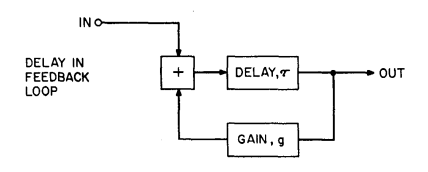
\includegraphics[width=%
0.50\textwidth]{dfl}
\caption{Delay all'interno di un feedback}
\label{fig:dfl}
\end{figure}

Dato che l'obiettivo è quello di produrre un elevato numero di echi a partire da un numero contenuto di oggetti, inseriamo dunque la linea di ritardo in un feedback avente come moltiplicatore $(g) < 1$.
Il risultato sarà un segnale che decade di $g$ volte ad ogni ciclo.

\begin{figure}[htp]
\centering
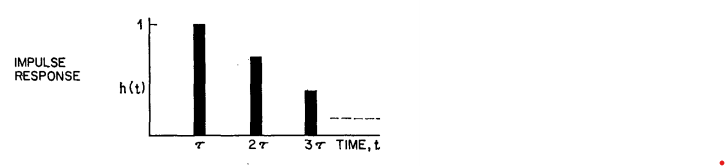
\includegraphics[width=%
0.60\textwidth]{dflir}
\caption{risposta in ampiezza}
\label{fig:dflir}
\end{figure}

La sua risposta in frequenza invece, presenta in modo periodico picchi e valli sullo spettro, aventi come valori rispettivamente $(1+g)$ e $(1-g)$. L’autore, data la somiglianza ad un pettine, rinomina il ciclo sopra descritto \emph{Comb Filter}, e così mi riferirò al medesimo d’ora in avanti.

\begin{figure}[htp]
\centering
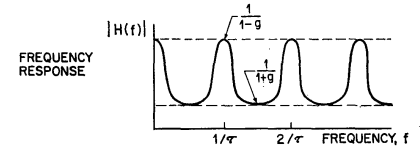
\includegraphics[width=%
0.50\textwidth]{dflspectrum}
\caption{}
\label{fig:dflspectrum}
\end{figure}

Questo comportamento del filtro comporta però una certa non esattezza in termini di spettro che Schroeder cerca di evitare, raffinando l’algoritmo tramite successive integrazioni.
La soluzione proposta dall’autore e Logan è il missaggio del suono diretto moltiplicato per $(-g)$ e il suono riverberato moltiplicato per $(1-g^2)$. Questo comporta una risposta piatta per tutte le frequenze. Il filtro risultante, chiamato \emph{All Pass Filter}, è descritto secondo il seguente schema e per le successive integrazioni, viene utilizzato come unità riverberante di base.

\begin{figure}[htp]
\centering
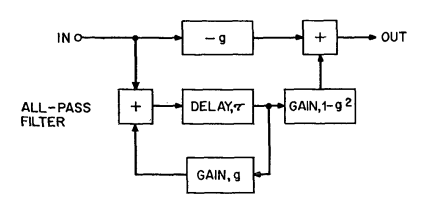
\includegraphics[width=%
0.50\textwidth]{apf}
\caption{All Pass filter di Schroeder}
\label{fig:apf}
\end{figure}

Per risolvere la problematica della densità degli echi, la soluzione di schroeder è quella di connettere in serie più riverberatori, in modo tale che la densità cresca in modo frattale per ogni unità connessa. Dato che abbiamo risolto il problema di una possibile colorazione del filtro, possiamo non preoccuparci che questo avvenga per una connessione in serie.

\begin{figure}[htp]
\centering
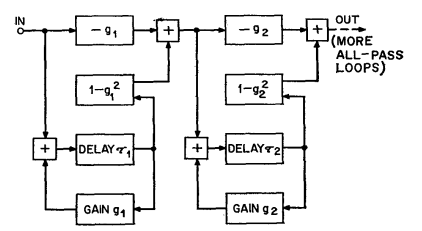
\includegraphics[width=%
0.50\textwidth]{apfseq}
\caption{sequenza di 5 All Pass}
\label{fig:apfseq}
\end{figure}

La densità che si cerca di raggiungere, ovvero quella di circa 1000 echi al secondo, è facilmente raggiungibile con 5 riverberatori in serie (il numero prodotto è di circa 810). A differenza di Schroeder abbiamo a disposizione molte più risorse, in termini di potenza di calcolo infatti possiamo serializzare molti più riverberatori e raggiungere un numero di riflessioni elevatissimo.

Successivamente, avendo constatato l’efficienza del riverberatore All Pass, Schroeder cerca di implementare alcune caratteristiche della riverberazione naturale.

Esse sono:

\begin{itemize}
\item Missaggio del suono diretto con il suono riverberato, senza alterare la struttura di All Pass;
\item Inserimento di un leggero sfasamento temporale tra, appunto, il segnale diretto e il segnale riverberato, dato che come sappiamo, il suono diretto raggiunge l’ascoltatore prima delle riflessioni;
\item La dipendenza alle frequenze del tempo di riverbero;
\end{itemize}

Il segnale non riverberato restituito dalla sequenza di all-pass risulta parecchio ininfluente, per questo Schroeder consiglia di moltiplicare per ($-g$) e sommare il segnale diretto proprio con questa serie, come illustrato in figura \ref{fig:apfmix}.

\begin{figure}[htp]
\centering
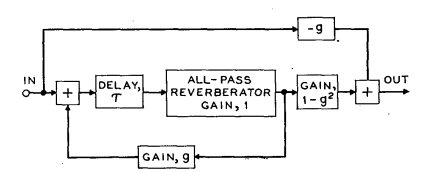
\includegraphics[width=%
0.50\textwidth]{apfmix}
\caption{sequenza di All Pass con aggiunta di segnale diretto}
\label{fig:apfmix}
\end{figure}

Il box chiamato \emph{“All-pass reverberator”} contiene, come detto, la serie di All Pass, inserito all’interno di un ulteriore feedback loop.
Da notare il delay iniziale, il quale permette un ritardo rispetto al suono diretto, rifornendo anche il secondo punto.

\bigskip

Un ultimo aspetto da considerare dell’articolo,  è l’utilizzo combinato di filtri Comb e All-pass per ricercare, al contrario dell’obiettivo originale, una risposta frequenziale altamente irregolare, come nel caso delle stanze reali.
In seguito agli esperimenti condotti ai Bell Telephone Laboratories, in cui si è scoperto che ad alte densità di riflessioni le irregolarità sono impercettibili, si è pensato di ricostruire l’algoritmo in modo tale da ricreare le condizioni di una stanza reale.
Lo schema è raffigurato in figura \ref{fig:comballpass}
\smallskip

\begin{figure}[htp]
\centering
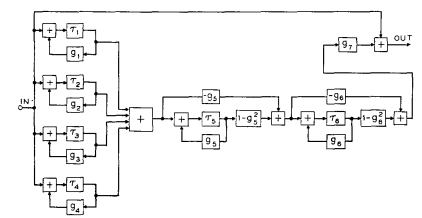
\includegraphics[width=%
0.60\textwidth]{comballpass}
\caption{Configurazione Comb-All Pass}
\label{fig:comballpass}
\end{figure}

Questa nuova configurazione conformazione prevede:
\begin{itemize}
\item Un certo numero di Filtri Comb, aventi tempi di delay incommensurabili oppure primi, connessi in parallelo. Questi filtri produrranno le cosiddette “Early reflections";
\item Un certo numero di All-Pass connessi in serie, in modo tale da incrementare la densità degli echi.
\item Al tutto verrà aggiunta una quantità di segnale diretto come nelle precedenti iterazioni.
\end{itemize}

\section{Articolo di Moorer}
Un successivo studio sulla simulazione digitale dei riverberi è stato condotto da \emph{James A. Moore} intorno al 1979, pubblicando i suoi risultati  su Computer Music Journal ,Vol. 3, No. 2.
L’articolo, intitolato \emph{“About this Reverberation Business”}, tratta di ulteriori integrazioni e accorgimenti che possono essere applicati durante lo sviluppo di un riverbero.

L’autore, infatti, partendo dalla letteratura già presente, tra cui gli articoli di Schroeder e J.Chowning, sperimenta nuovi algoritmi, rendendo più snelli i precedenti, sempre tendendo ad una realisticità del riverbero.

Innanzitutto vengono ripresi i sistemi fondamentali dell’analisi di Schroeder, vale a dire, il filtro Comb (visto in figura \ref{fig:dfl}) e il filtro All Pass (visto in figura \ref{fig:apf}). Quest’ultimo in una seconda versione caratterizzata da una singola moltiplicazione, a fronte delle 3 precedenti, rendendolo più sostenibile a livello di computazione.

\begin{figure}[htp]
\centering
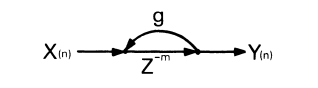
\includegraphics[width=%
0.60\textwidth]{combmoorer}
\caption{Filtro Comb di Moorer}
\label{fig:combmoorer}
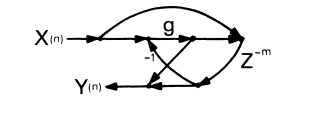
\includegraphics[width=%
0.60\textwidth]{apfmoorer}
\caption{Filtro All Pass di Moorer}
\label{fig:apfmoorer}
\end{figure}

Aventi le seguenti funzioni di trasferimento:
\begin{equation}
T(z) = \frac{g + z^{-m}}{1+gz^{-m}}
\end{equation}
\begin{equation}
T(z) = \frac{z^{-m}}{1-gz^{-m}}
\end{equation}

Osservando la funzione trasferimento dell’All Pass possiamo notare come il coefficiente del numeratore sia in ordine inverso di quello al denominatore, forzando gli zeri ad essere reciproci dei poli, definendo il comportamento All Pass del filtro.

Seguendo il lavoro fatto da Schroeder, per utilizzare i sistemi come riverberatori è necessario utilizzare una combinazione degli stessi.

Le combinazioni sono le medesime viste in precedenza e proposte da Schroeder (fig \ref{fig:apfseq} e \ref{fig:comballpass}). Parliamo dunque di una serie di All Pass nel primo algoritmo e, una cascata di comb filter seguiti da 2 All Pass nel secondo

\begin{figure}[htp]
\centering
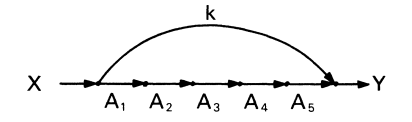
\includegraphics[width=%
0.60\textwidth]{allallpass}
\caption{Filtro Comb di Moorer}
\label{fig:allallpass}
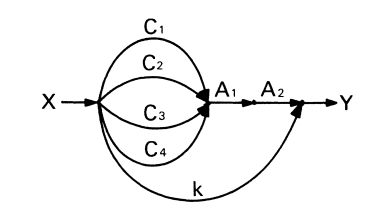
\includegraphics[width=%
0.60\textwidth]{comballpassmoorer}
\caption{Filtro All Pass di Moorer}
\label{fig:comballpassmoorerB}
\end{figure}

\subsection{Problematiche Del riverberatore}

Il riverberatore così ottenuto, però, non rispecchia alcune caratteristiche desiderate, portando ad aberrazioni acustiche non presenti in natura.
Le problematiche riscontrate possono essere riassunte in:

\begin{itemize}
\item riverberazione non ottimale per suoni impulsivi e con transienti molto corti, producendo pattern ritmici composti dagli echi al posto di un riverbero uniforme;
\item riverberazione con un carattere metallico, soprattutto per tempi molto lunghi;
\end{itemize}

A questo punto l’autore considera l’utilizzo di nuove unità riverberanti, ma comunque mantenendo la struttura Comb-All Pass, ritenuta la migliore in termini di risposta.

\subsection{Nuove unità riverberanti}

Nel corso delle sue sperimentazioni Moorer costruisce altre 4 unità riverberanti, alcune molto simili tra di loro in quanto i concetti alla base restano i medesimi. In particolare, l’intuizione dell’autore è stata quella di introdurre un ulteriore filtro all’interno dei feedback.

Lo scopo del filtro, ricollegandoci agli argomenti trattati nei capitoli precedenti, è quello di simulare l’attenuazione delle alte frequenze causate dall’aria. Come già detto, è un coefficiente che, in base a caratteristiche quali umidità e temperatura, sottrae energia alle alte frequenze dello spettro, scurendo quest’ultimo.

\subsection{Nuove unità riverberanti}

Come detto, le unità proposte sono 4, ma una in particolare sembra essere la più efficiente, ovverosia:

\begin{figure}[htp]
\centering
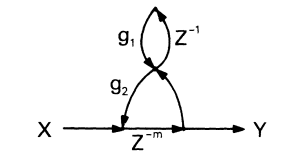
\includegraphics[width=%
0.50\textwidth]{combfiltro}
\caption{Filtro Comb con all'interno un filtro Passa Basso}
\label{fig:combfiltro}
\end{figure}

Come è possibile notare, si tratta di un Comb filter al cui interno è presente un filtro di tipologia Low pass $T(z)$. Il valore di $g_1$ controlla il roll-off del filtro e in seguito troveremo un modo per capire quale valore sarà più conveniente.
All’interno, i valori $g_1$ e $g_2$ seguiranno la condizione di $g_1+g_2<1$ per motivi di stabilità.

La risposta in frequenza, a detta di Moorer,  non sarà in grado di restituire un valore coerente alla realtà, in quanto il singolo filtro Low pass (di primo ordine) è un compromesso per rendere il tutto più efficiente.

Successivamente, nell’articolo viene anche consigliato di tenere in considerazione della modifica dei tempi di delay in base alle caratteristiche dell’aria (temperatura e umiditá), anche se nel testo si fa riferimento a valori standard e non modificabili.
I valori di $g$, dipendenti dall’umidità, sono in seguito esposti grazie agli studi di Moorer nel seguente grafico.
\begin{figure}[h!]
\centering
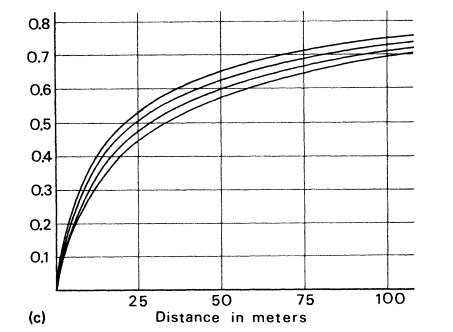
\includegraphics[width=%
0.50\textwidth]{assorbimentomoorer}
\caption{Grafico raffigurante l'andamento del valore di $g$ a causa dell'assorbimento dell'aria}
\label{fig:assorbimentomoorer}
\end{figure}
\bigskip
\subsection{In conclusione}
Moorer conclude la sezione riportando i risultati ottenuti. L’inserimento del filtro permette una miglior riverberazione per i suoni impulsivi, infatti il tempo di ogni eco risulta essere esteso, soprattutto per quanto riguarda le prime riflessioni e nascondendo i vuoti creati dalla bassa densità.
Il risultato sonoro non è particolarmente entusiasmante a detta dell’autore, ma sopperisce ad alcune mancanze delle precedenti iterazioni, rendendo questo sistema il più efficace al momento della scrittura.
